\section{Introduction}
It is a well known fact that a vehicle driving at a constant velocity use less fuel than an accelerating vehicle due to the physical laws of motion\cite{Vejdir}.
In order to save fuel, one should therefore try to drive with a constant speed, but several factors prevents drivers in doing this. 
These factors are for example merging roads, blocking vehicles, traffic incidents and traffic lights. 
It is esimated that 1.8 bilion danish kroner is lost on fuel each year because of vehicles stopping in traffic lights in Denmark \cite{Vejdir}.

Traffic lights hinders the flow of traffic as it blocks vehicles arriving from one direction in order to allow other vehicles to drive through the intersection.
Normally, a driver will only be able to guess when the light is going to change based on local knowledge of the area. 
Looking at Figure \ref{fig:Introduction:network} vehicle $\veh_2$ is approacing the intersection.
Now assume that vehicle $\veh_2$ knows the distance $\dist_3$ where he has to stop for the traffic light. 
Then also assume that vehicle $\veh_2$ knows that in at least $4$ seconds the traffic ligth will change to green. 
Then it is posible to calculate at which speed $\veh_2$ should drive such that it will drive the distance $\dist_3$ in at least $4$ seconds. 
Now by the time the vehicle reaches the intersection the signal will have changed and a full stop is avoided.
\begin{figure}[htb]
\centering
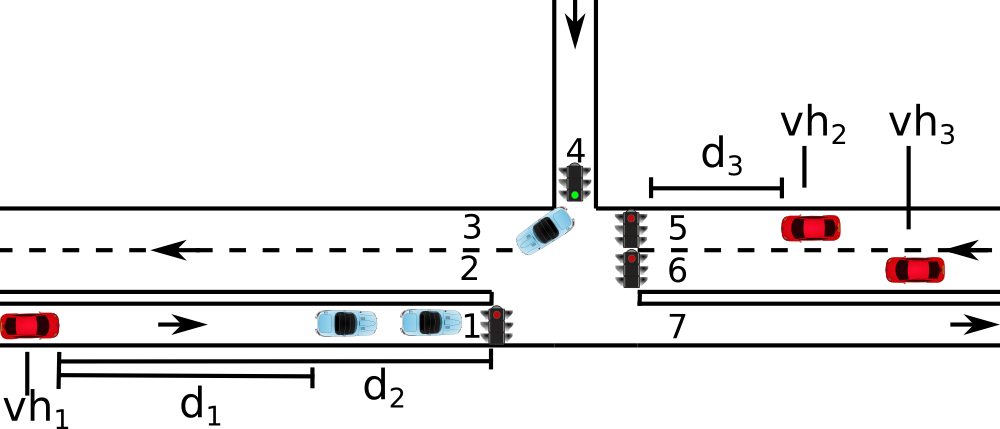
\includegraphics[width=0.45\textwidth]{../images/introNetwork.png}
\caption{Example network}
\label{fig:Introduction:network}
\end{figure}

Road authorities try to design traffic lights such that the flow of traffic is maximised in all directions.
This can be very difficult, especially in junctions with changing traffic density through out the day.
Two main techniques are used for traffic lights: pretimed traffic controllers, where the signals loop between red, yellow and green in a predefined pattern; and traffic actuated controllers, where approacing vehicles are detected by road-side detectors such that the signals can be adjusted to the current traffic flow.
A combination of the two is often used.
The cost of upgrading a traffic light with detectors is 200.000-300.000 danish kroner, not counting extra maintenance costs to repair broken detectors\cite{Vejdir}.

We focus on investigating whether it is possible to reduce the fuel consumption at traffic ligths by matching driving speed to traffic lights. 
We investigate this through simulations with real world map data, traffic data and traffic light programs. %TODO check we do this
We use the traffic simulator SUMO (Simulation of Urban Mobility)\cite{sumo} interfaced via TraCI (Traffic Control Interface)\cite{traci} which is a full scall microscopic traffic simulator.

The system that we propose, is designed with the assumption that very few vehicle will be using it initialy. 
Because of this, we cannot rely on communication between vehicles.
We do, however, assume that traffic lights and vehicles can communicate such that the phases of the traffic lights are avaiable.
We assume the vehicles use a GPS system that handels the communication and that provides a route to travers.
We do not require any further equipment that this.
Additionally, we assume that all drivers follow the rules of traffic, e.g. drives below the speed limit, do not drive into other vehicles and wait for crossing traffic.

%TODO: Challenges
\begin{enumerate} %TODO: More challenges?
\item \textbf{Limitations of SUMO.}
Simulators do not simulate the the real world perfectly, and some simplefications are made in order for it to function. 
These include, limits on the size of the road network, lack of pedestians, wether factors and more, simplified acceleration and deceleration profiles and the ability to break the traffic rules.
\item \textbf{Configuring SUMO.}
The simulations should be as realistic as possible, and therefore based on real data. 
The road network should have the same dimensions, the traffic signals should behave similar and the congestion levels should be similar to what is observed in the real world.
\item \textbf{No communication between vehicles.} 
The system should work even though very few vehicles are using it initially, and hence we cannot rely on communication between vehicles. 
The number of blocking vehicles in the road network, will therefore be an unknown factor in the system.
\end{enumerate}

%TODO: Contributions

The structure of the remaining paper is as follows: 
We describe the related work in Section~\ref{sec:RelatedWork} and our model in Section~\ref{sec:Model}. 
In Section~\ref{sec:Math}, we detail the proposed techinique by going through the algorithm.
Section~\ref{sec:UseCase} is about the use case that we test the proposed technique on, and the results of these tests are evaluated in Section~\ref{sec:Test}. 
We conclude the findings in Section~\ref{sec:Conclusion}.





